\documentclass[acmsmall,screen]{acmart}
\setcopyright{none}
\copyrightyear{2023}
\acmYear{2023}
\acmDOI{}

\citestyle{acmauthoryear}

\usepackage{fancyhdr}
\usepackage{fancyvrb}
\usepackage{algpseudocode}
\usepackage{algorithm}
\usepackage{graphicx}
\usepackage{wrapfig}
\begin{document}

\title{Bottom-Up Enumerative Synthesis of Recursive Programs using Generalized Folds}

\author{Rafaello Sanna}
\author{Nada Amin}
\affiliation{%
  \institution{Harvard University}
  \country{USA}
}
\author{William Byrd}
\affiliation{%
  \institution{University of Alabama at Birmingham}
  \country{USA}
}

\renewcommand{\shortauthors}{Raffi Sanna, Nada Amin and Will Byrd}

\settopmatter{printacmref=false}
\settopmatter{printfolios=true}
\renewcommand\footnotetextcopyrightpermission[1]{}
\pagestyle{fancy}
\fancyfoot{}
\fancyfoot[R]{CS252R (Fall 2023)}
\fancypagestyle{firstfancy}{
  \fancyhead{}
  \fancyhead[R]{CS252R (Fall 2023)}
  \fancyfoot{}
}
\makeatletter
\let\@authorsaddresses\@empty
\makeatother

\begin{abstract}
    We present DAN, a new technique for extending bottom-up enumerative synthesis to recursive procedures. Bottom-up synthesis has been shown its ability to generate non-trivial programs in many interesting domains, and exploits the problem's overlapping subproblems and optimal substructure. However, these properties are not available in the cases of recursive programs, where subproblems are often not defined. One solution to this problem is to build up recursive programs from smaller sub-problems, exploiting the structure of recursive data structures to guide the recursion itself, often by using a library of recursive functions known to be terminating. We extend this work to arbitrary data structures, using techniques from the generic programming and structured recursion literature.
\end{abstract}

\keywords{Program Synthesis, Recursion Schemes, Generic Programming}

\maketitle
\thispagestyle{firstfancy}

\section{Introduction}

Program synthesis has shown the potential to revolutionize the task of programming. It allows programmers to express the program they want in a simple, but often ambiguous manner, and have the machine do the work of finding a program that fits their specification. A canonical example of this has been the task of programming-by-example (PBE), in which a user specifies a general transformation by demonstrating it on a series of concrete input/output pairs (IO pairs). The role of a programming-by-example system is to learn the underlying transformation from the examples and render it as program code which can be applied to any object.

\subsection{Bottom-Up Synthesis}

One of the most successful methods of program synthesis has been bottom-up synthesis, which enumerates possible values in the language by the size of the smallest expression which produces them. We start first with the constants of the language and the inputs from the user, each of these with size zero. We then grow our set of values by applying the language's operators to each of the values we've seen so far, then keeping all the new values we find, along with the programs that created them. As the set of possible values grows, we eventually reach the values we want to generate. The program which generates these values is then the one specified by the user. The major advantage of bottom-up synthesis is that we work with values, not programs. This is a classic example of overlapping substructure - there are many programs which generate the same value, so we can share repeated work by keeping track only one canonical program for every value.

\newcommand*\OR{\ |\ }

\begin{figure}[h]
\begin{align*}
  t & \to 0 \OR 1 \OR ... \\
    & \OR x \\
    & \OR t + t \OR - t \OR t * t \OR ( t ) \\
    & \OR \texttt{Y}(x. t) \\
    & \OR \texttt{if} \ t\ \texttt{then}\ t\ \texttt{else} \ t\
\end{align*}
\caption{A Simple Language with the Fix-Point Combinator}
\label{fig:mathWithRec}
\end{figure}

\subsection{Partial Operators and the Fix-Point Combinator}

The major upside of bottom-up synthesis is also its downside. While all values have programs which evaluate to them, in many languages, not all programs evaluate to values. Operators in these language are called partial - they can only sometimes be meaningfully evaluated. One operator which is of this kind is the fix-point combinator of language \ref{fig:mathWithRec}, written as the term \verb|Y(x.t)|, which evaluates its body \verb|t| with the variable \verb|x| bound to \verb|Y(x.t)|. This operator expands the set of possible programs which can be expressed, but also introduces many programs which do not meaningfully terminate. For example, the only possible reduction step in the evaluation of the term \verb|Y (rec. rec)| is \verb|Y (rec. rec)|. When combined with a conditional operator such as \verb|if-then-else|, it makes the language Turing complete, meaning we cannot meaningfully check if a program terminates.

\section{Related Work}

The most common solution to the problem of non-terminating programs is to introduce a full recursive operator such as \verb|Y|, but restrict its use only to certain special cases[1][2]. For instance, in the ESCHER[2] tool, the \verb|Y| operator can only be generated when the recursion is shown to be structural, as in many languages with totality checkers. The advantage of techniques such as this one is that the language comes more naturally to humans. Most programmers do not worry about totality checking in their day-to-day work, so the ability to express non-terminating procedures is natural (for this reason, many papers reformat their examples to remove the \verb|Y| combinator altogether, showing a more traditional recursive definition form). The major disadvantage is that we lose the overlapping substructure of the original problem. The value of a term (indeed, whether or not it even \textit{has} a value) is a function not only on its free variables, but on its location within the program as a whole. This requires the generation of partial programs which take on different (or no) values when evaluated in different areas of the program.

The alternative method to this is to break down the recursion into smaller parts, each of which can be solved using non-recursive code[3]. An illustrative example of this method is the $\lambda^2$[3] project. Rather than using a language with a possibly non-terminating fix-point combinator, it enumerates terms using higher-order procedures typical of functional programming, such as \texttt{map}, \texttt{filter} and \texttt{fold}. These procedures allow for natural, inductive transformations on functional data structures, while still ensuring the language is terminating. The major downside of this approach is that it requires a complete set of such combinators in advance. It isn't possible, for example, to define new data structures or new operators on existing data structures. 

We expand prior work by performing true bottom-up synthesis on arbitrary data structures. To achieve this, we use generic programming and recursion schemes to derive operators such as \texttt{fold} automatically.

\section{Generalized Folds}

The \texttt{fold} procedure for lists is well-known by functional programmers[4]. However, its application to recursive data-structures (and the ability for such folds to be defined automatically) is not. Recall the definition of \texttt{List}s and their fold:

\begin{verbatim}
data List a = Cons a (List a)
            | Nil

foldList : (onCons : el -> acc -> acc) -> (onNil : acc) -> List el -> acc
foldList onCons onNil = rec
  where
    rec : List el -> acc
    rec Nil = onNil
    rec (Cons x xs) = onCons x (rec xs)
\end{verbatim}

There's a clear correspondence between the parameters of the fold and the constructors in the datatype. For each constructor, the fold takes a procedure which takes the fields of the constructor as arguments and returns a new accumulated value. We essentially define our own interpretation of each constructor, then recursively apply it throughout.

Consider the definition of the following algebraic datatype for representing compound objects:

\begin{verbatim}
data Obj = Zero
         | Succ Obj
         | Nil
         | Cons Obj Obj
\end{verbatim}

We can try writing a fold in the same way: mapping each constructor to a parameter, then combining them.

\begin{Verbatim}
foldObj : (onZero : Obj) ->
          (onSucc : Obj -> Obj) ->
          (onNil : Obj) ->
          (onCons : Obj -> Obj -> Obj) ->
          Obj -> Obj
foldObj onZero onSucc onNil onCons = rec
  where
    rec : Obj -> Obj
    rec Zero = onZero
    rec (Succ x) = onSucc (rec x)
    rec Nil = onNil
    rec (Cons x y) = onCons (rec x) (rec y)
\end{Verbatim}

\section{Deriving Folds for Program Synthesis}

These generalized folds are the key to synthesis in Dan. Each program is represented as a fold over the datatype of interest, and each case of the fold is structured as a subproblem which can be solved independently. 

\begin{wrapfigure}{l}{5.5cm}
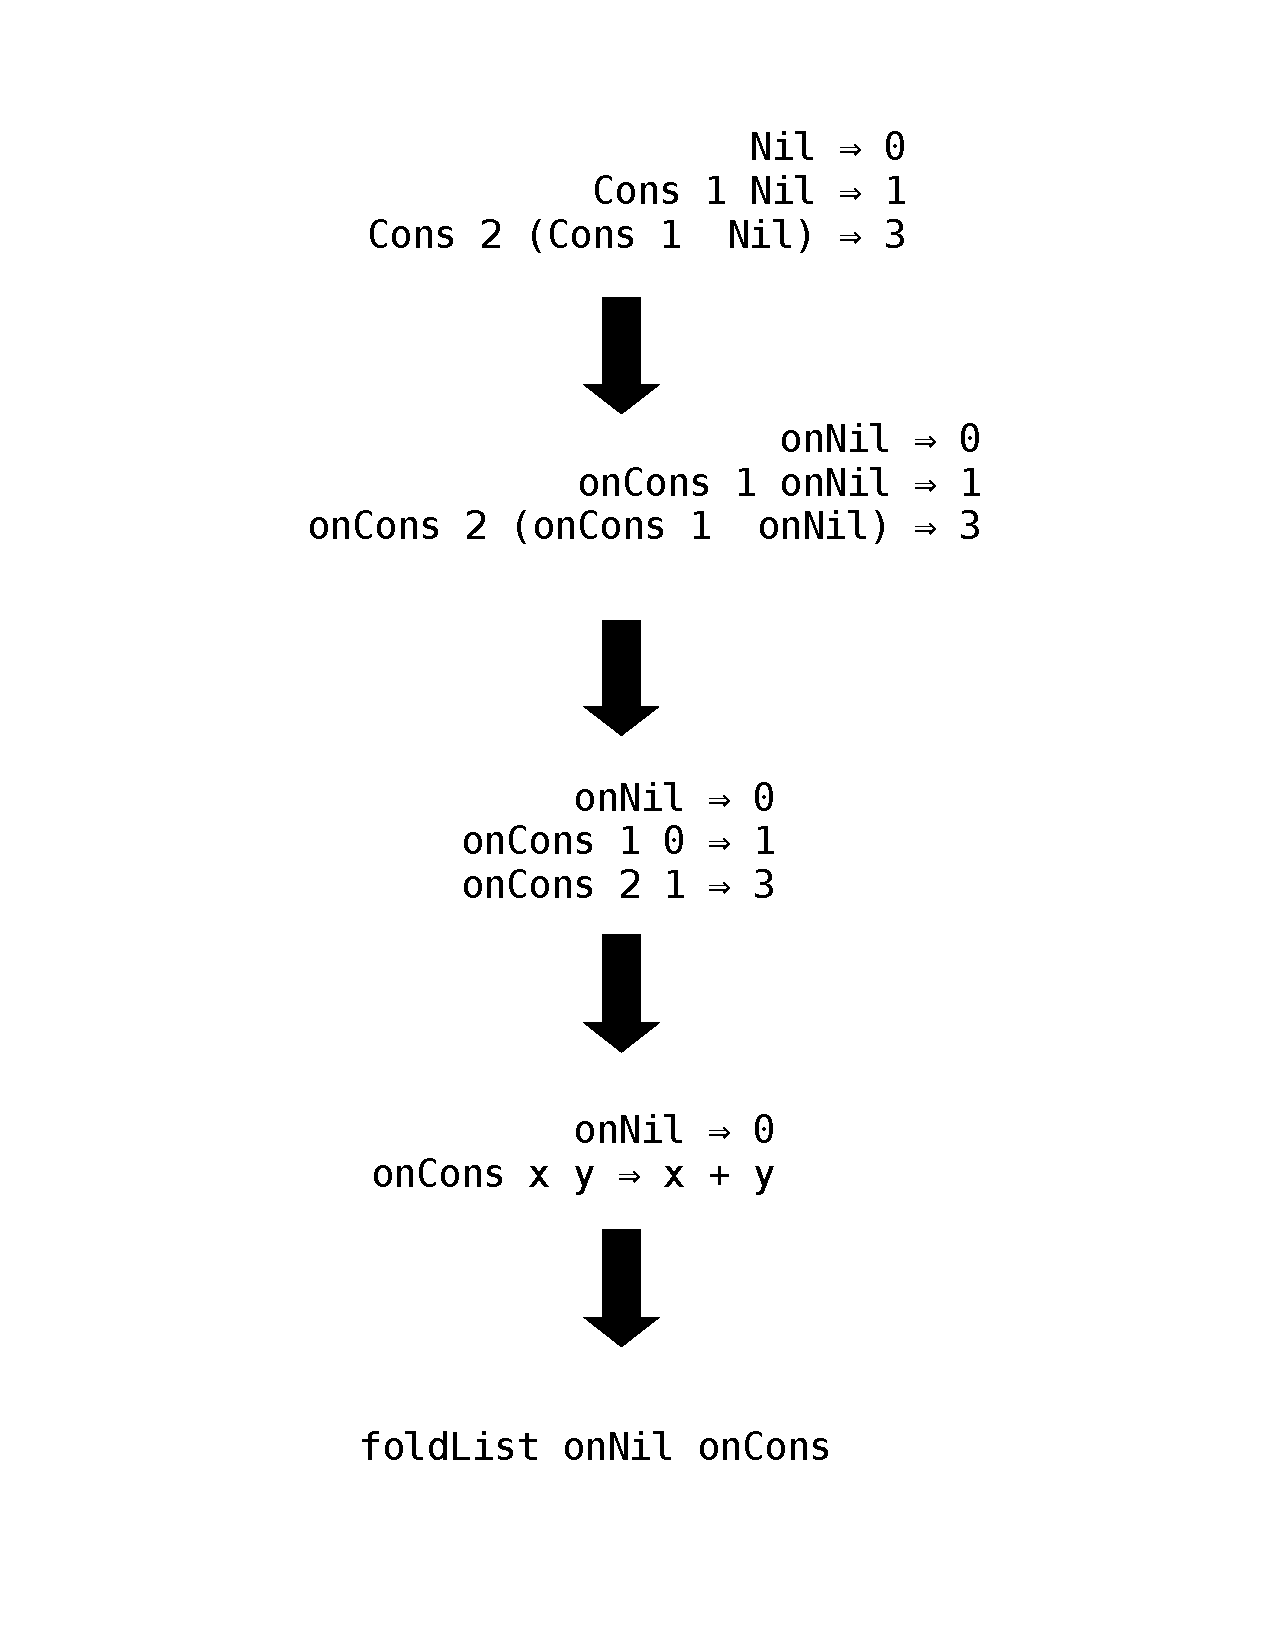
\includegraphics[width=0.4\textwidth]{Diagram.pdf}
\end{wrapfigure}

For each constructor of the datatype being folded over, Dan creates an individual procedure for solving that case of the recursion. The examples are then split up depending on the constructor of the argument. For constructors with recursive fields, the recursive structures are replaced with the result of the recursion on those structures. We then have a set of input-output examples which can be solved by an off-the-shelf bottom-up synthesis algorithm. Finally, each of the generated procedures is joined together into the fold.

\section{Future Work}

Immediate next steps forwards for the Dan project would be expanding the implementation. Currently, it can only generate dynamically typed programs - all terms must be of a single type. This works, but limits the opportunities for pruning possible programs and makes expressing problems in the implementation language awkward. Another major improvement would be expressing new kinds of recursion other than \texttt{fold}, and defining multiple implementations of \texttt{fold} for different datatypes.

It would also be helpful to further develop the connection between Dan and its category-theoretic notions. Currently, the only scheme provided is a catamorphism, but providing options such as a paramorphism or hyglomorphism would extend its synthesis abilities significantly.

Lastly, Dan needs to be evaluated more thoroughly, both in isolation and compared to other tools, such as ESCHER and $\lambda^2$. Becoming competitive with these projects may require some performance engineering, as the current implementation was written primarily for ease of reading and experimentation.

\begin{acks}
    I would like to thank Nada Amin and William Byrd for their initial ideas for and implementation of this project. They have been a fantastic help both within 252R and without. I'd also like to thank Nada (again) and Tyler Holloway for teaching the class this semester. It's been incredibly engaging and has lead me to meet several interesting new people. I'd also like to thank the other members of the class for their great presentations, both of their work and their own, and comments about presented work, keeping the class interactive and inquisitive. I'd finally like to thank Dan Friedman, after whom the project is named, for his teaching style, which inspired the technique itself.
\end{acks}

\section*{References}

\begin{enumerate}
  \item Peter-Michael Osera and Steve Zdancewic. 2015. Type and Example Directed Program Synthesis. SIGPLAN Not. 50, 6 (June 2015), 619–630. https://doi.org/10.1145/2813885.2738007
  \item Albarghouthi, Aws and Gulwani, Sumit and Kincaid, Zachary. 2013. Recursive Program Synthesis. Proceedings of the 25th international conference on Computer Aided Verification. CAV'13. https://www.microsoft.com/en-us/research/publication/recursive-program-synthesis/
  \item John K. Feser, Swarat Chaudhuri, and Isil Dillig. 2015. Synthesizing data structure transformations from input-output examples. SIGPLAN Not. 50, 6 (June 2015), 229–239. https://doi.org/10.1145/2813885.2737977
  \item Jeremy Gibbons and Oege de Moor. 2003. The Fun of Programming. Palgrave. 41-60.
\end{enumerate}
\end{document}

% LocalWords:  subproblems
